\documentclass[portuguese]{sbc2025}%

\usepackage[misc,geometry]{ifsym}

\raggedbottom  % Prevent underfull vbox warnings

\usepackage{aas_macros}
\usepackage[bottom]{footmisc}

\usepackage{tabularray}
\usepackage{adjustbox}
\usepackage{stfloats}
\usepackage{placeins}
\usepackage{float}
\usepackage{tikz}
\usetikzlibrary{arrows.meta,positioning,fit,calc,matrix}

\usepackage{afterpage}
\usepackage{url}
\usepackage{pifont}

\setcitestyle{square,comma}

\definecolor{engtitle}{rgb}{0.5,0.5,0.5}
\definecolor{orcidlogo}{rgb}{0.37,0.48,0.13}
\definecolor{unilogo}{rgb}{0.16, 0.26, 0.58}
\definecolor{maillogo}{rgb}{0.58, 0.16, 0.26}
\definecolor{darkblue}{rgb}{0.0,0.0,0.0}
\hypersetup{colorlinks,breaklinks,
            linkcolor=darkblue,urlcolor=darkblue,
            anchorcolor=darkblue,citecolor=darkblue}

\jyear{2025}

\category{Artigo de Pesquisa/Research Paper}
\title[Sistema de Monitoria-IC: Plataforma Web para Gestão de Monitorias Acadêmicas da UFBA]{Sistema de Monitoria-IC: Plataforma Web para Gestão Completa de Monitorias Acadêmicas da UFBA}
\engtitle{\textcolor{engtitle}{Sistema de Monitoria-IC: Web Platform for Complete Management of Academic Monitoring Programs at UFBA}}

\author[Sena et al. 2025]{
\affil{\textbf{Luis Felipe Cordeiro Sena}~\orcidlink{0009-0009-3997-3639}~\textcolor{blue}{\faEnvelopeO}~~[{Universidade Federal da Bahia}~|\href{mailto:luis.sena@ufba.br}{~{\textit{luis.sena@ufba.br}}}~]}

\affil{\textbf{Frederico Araújo Durão}~\orcidlink{0000-0002-7766-6666}~~[{Universidade Federal da Bahia}~| \href{mailto:fdurao@ufba.br}{{\textit{fdurao@ufba.br}}}~]}
}

\begin{document}

\begin{frontmatter}

\maketitle

\begin{mail}
Instituto de Computação, Universidade Federal da Bahia, Av. Milton Santos, s/n - Campus de Ondina, PAF 2, Salvador, BA, 40170-110, Brasil.
\end{mail}

\begin{abstract-pt}
A monitoria acadêmica é um processo fundamental nas universidades brasileiras que permite aos alunos desenvolverem habilidades pedagógicas enquanto auxiliam no processo de ensino-aprendizagem. Porém, o gerenciamento desse processo frequentemente enfrenta desafios relacionados à burocracia, falta de transparência e múltiplos processos manuais ineficientes. Este trabalho apresenta o desenvolvimento do Sistema de Monitoria-IC, uma plataforma Web projetada para automatizar e simplificar o ciclo de vida dos projetos de monitoria na UFBA. A solução proposta digitaliza desde a criação e assinatura de projetos pelos professores até a aprovação administrativa e geração de planilhas consolidadas para envio ao Instituto/PROGRAD. O sistema foi desenvolvido utilizando tecnologias modernas como Next.js 15, TypeScript, tRPC, PostgreSQL e MinIO, seguindo princípios de engenharia de software que garantem escalabilidade e manutenibilidade. A arquitetura implementada separa claramente as responsabilidades entre um Sistema de Processamento de Transações (SPT) para operações cotidianas e funcionalidades gerenciais para análise e controle. A validação técnica através de testes end-to-end demonstra a robustez da solução. Os resultados esperados indicam que a automação proposta tende a eliminar retrabalho administrativo, aumentar a transparência por meio de histórico auditável e estabelecer uma base sólida para a modernização da gestão acadêmica na universidade.
\end{abstract-pt}

\begin{abstract-en}
Academic monitoring is a fundamental process in Brazilian universities that allows students to develop pedagogical skills while assisting in the teaching-learning process. However, managing this process often faces challenges related to bureaucracy, lack of transparency, and multiple inefficient manual procedures. This work presents the development of Sistema de Monitoria-IC, a web platform designed to automate and simplify the lifecycle of monitoring projects at UFBA. The proposed solution digitizes the process from project creation and signing by professors to administrative approval and generation of consolidated spreadsheets for the Institute/PROGRAD. The system was developed using modern technologies such as Next.js 15, TypeScript, tRPC, PostgreSQL, and MinIO, following software engineering principles that ensure scalability and maintainability. The implemented architecture clearly separates responsibilities between a Transaction Processing System (TPS) for daily operations and managerial functionalities for analysis and control. Technical validation through end-to-end tests demonstrates the solution's robustness. Expected results indicate that the proposed automation tends to eliminate administrative rework, increase transparency through auditable history, and establish a solid foundation for modernizing academic management at the university.
\end{abstract-en}

\begin{pchaves}
Gestão Acadêmica, Sistema de Monitoria, Arquitetura de Software, Desenvolvimento Web, Automação de Processos.
\end{pchaves}

\begin{keywords}
Academic Management, Monitoring System, Software Architecture, Web Development, Process Automation.
\end{keywords}

\begin{dates}
% Informações serão preenchidas pelo editor antes da publicação
\end{dates}

\end{frontmatter}

\section{Introdução}
\label{sec:intro}

A monitoria acadêmica representa um dos pilares fundamentais do ensino superior brasileiro, estabelecendo-se como uma prática pedagógica que beneficia simultaneamente monitores, estudantes e docentes. Regulamentada pela Lei nº 9.394/96 (Lei de Diretrizes e Bases da Educação Nacional), a monitoria permite que alunos com destacado desempenho acadêmico auxiliem seus pares no processo de aprendizagem, desenvolvendo competências didáticas enquanto aprofundam seus conhecimentos na disciplina \cite{Brasil1996}.

Na Universidade Federal da Bahia (UFBA), o programa de monitoria segue um fluxo complexo que envolve múltiplos atores e etapas interdependentes. O processo inicia-se com o planejamento semestral, quando a administração importa dados de disciplinas e professores. Em seguida, os docentes criam e submetem projetos de monitoria que precisam ser aprovados administrativamente. Após a aprovação, ocorre a publicação de editais internos, inscrição de candidatos, processo seletivo, alocação de bolsas, e finalmente, a consolidação de dados para envio à PROGRAD (Pró-Reitoria de Graduação).

A literatura de Sistemas de Informação fornece evidências de que a digitalização e a automação de processos reduzem custos transacionais, eliminam retrabalho e aumentam a confiabilidade e a auditabilidade dos registros \cite{Laudon_Laudon_2011, Davenport1993, Hammer1993}. Em contextos públicos e acadêmicos, iniciativas de governo digital e transformação digital têm sido associadas a ganhos de eficiência administrativa e transparência, desde que apoiadas por arquitetura tecnológica moderna e governança de dados adequada \cite{WorldBank2022, UNESCO2023}. No escopo deste trabalho, tais fundamentos são adotados para sustentar a proposta de um sistema unificado de monitoria, substituindo fluxos fragmentados por um \textit{workflow} padronizado, rastreável e escalável.

Apesar de sua importância reconhecida, a gestão dos programas de monitoria na UFBA ainda depende predominantemente de processos manuais e fragmentados. Formulários em papel, planilhas eletrônicas dispersas, comunicação via e-mail e ausência de um sistema centralizado caracterizam o cenário atual, resultando em ineficiências operacionais significativas. Essa realidade contrasta com a tendência global de digitalização e automação de processos administrativos no ambiente acadêmico. \citet{Laudon_Laudon_2011} argumentam que a tecnologia da informação constitui uma das principais ferramentas para alcançar excelência operacional.

\subsection{Identificação do Problema}

O processo de monitoria na UFBA é lento, caro e opaco. Do lado docente, há retrabalho sistemático (recriação de projetos a cada semestre), dispersão de documentos (planilhas, PDFs e e-mails) e ausência de trilhas de auditoria --- combinação que consome horas de atividades-fim e eleva o risco de erro. A seleção permanece predominantemente manual e heterogênea entre departamentos, impedindo comparabilidade de critérios e produzindo falhas de registro.

Para estudantes, a descoberta de vagas é imprevisível e a jornada é fragmentada: múltiplos formulários, anexos por canais distintos e ausência de um painel único para acompanhar prazos, status e resultados --- o que reforça a percepção de opacidade e desestimula a participação.

Administrativamente, a consolidação de dados heterogêneos gera retrabalho, dificulta a conformidade com regulamentos e prazos e fragiliza a prestação de contas. Sem um repositório transacional e analítico integrado, relatórios custam caro e análises históricas confiáveis tornam-se inviáveis para decisões como distribuição de bolsas e avaliação de efetividade de projetos.

Em síntese, há uma lacuna tecnológica clara: falta um sistema de informação \textit{fim-a-fim} específico para monitoria que integre criação e aprovação de projetos, publicação de editais, inscrições, seleção, aceite de vagas e consolidações finais. A literatura indica que a automação e a padronização, apoiadas por arquitetura adequada e governança de dados, reduzem custos transacionais, retrabalho e erros e elevam a confiabilidade e a auditabilidade dos registros \cite{Davenport1993, Hammer1993, Laudon_Laudon_2011, WorldBank2022, UNESCO2023}.

\subsection{Objetivos}

Este trabalho documenta o desenvolvimento e implementação do Sistema de Monitoria-IC, uma plataforma Web completa para gestão dos projetos de monitoria do Instituto de Computação da UFBA. O objetivo central é substituir fluxos manuais e dispersos por um sistema único que garanta transparência, rastreabilidade e padronização de todo o processo de monitoria.

Os objetivos específicos incluem:

\begin{enumerate}
  \item Digitalizar o ciclo completo de projetos de monitoria: desde a criação com templates reutilizáveis, assinatura digital pelo professor, submissão, até aprovação administrativa e publicação de editais

  \item Automatizar o processo seletivo: permitindo inscrições online, captura automática de notas e CR do histórico, consideração de equivalências entre disciplinas, e publicação transparente de resultados

  \item Sistematizar a alocação de bolsas: com geração automática de planilhas para o Instituto, configuração do total de bolsas informado pela PROGRAD, e alocação por projeto com validações automáticas

  \item Eliminar trabalhos manuais repetitivos: através de automação de notificações por e-mail, geração de documentos PDF, e integração com armazenamento de arquivos

  \item Fornecer base analítica para tomada de decisões: com dashboards administrativos, APIs para integração, e relatórios consolidados para análises institucionais
\end{enumerate}

\subsection{Fora do Escopo}

Embora o sistema cubra o ciclo de vida completo da monitoria acadêmica, algumas funcionalidades foram deliberadamente excluídas do escopo deste trabalho. Primeiro, o módulo de relatórios finais e certificados (Fase 6 do fluxo de monitoria) foi especificado nos requisitos mas não implementado, sendo priorizado como trabalho futuro devido a restrições de tempo e à necessidade de validação do fluxo principal antes de sua expansão. Segundo, a integração automática com o sistema acadêmico institucional (SIAC ou SIGAA) para captura de históricos e notas permanece manual, exigindo que estudantes anexem documentos comprobatórios durante a inscrição. Terceiro, o sistema foi desenvolvido especificamente para o Instituto de Computação da UFBA, com adaptações necessárias para expansão a outros departamentos ou instituições. Quarto, funcionalidades de analytics avançado, como sistema de recomendação para correspondência entre aluno e projeto ou predição de desempenho com técnicas de aprendizado de máquina, foram identificadas como melhorias futuras mas não integradas nesta versão inicial. Por fim, um aplicativo móvel nativo não foi desenvolvido, embora a interface Web seja responsiva e funcione adequadamente em dispositivos móveis via navegador.

\subsection{Contribuições}

Este trabalho apresenta quatro contribuições principais para a área de Sistemas de Informação aplicados à gestão acadêmica. Primeira, propõe e implementa uma arquitetura em três camadas (Router-Service-Repository) específica para o domínio de monitoria acadêmica, demonstrando como separar responsabilidades entre apresentação, lógica de negócio e acesso a dados em um sistema transacional com múltiplos atores e requisitos formais de auditoria. Segunda, desenvolve um workflow automatizado completo que cobre as cinco primeiras fases do ciclo de monitoria (planejamento, aprovação, alocação, seleção e consolidação), incluindo funcionalidades inovadoras como templates reutilizáveis de projetos, assinaturas digitais integradas, consideração automática de equivalências curriculares e geração de documentos formais em PDF, resultando em redução estimada de 80\% no tempo gasto em tarefas administrativas repetitivas. Terceira, documenta um estudo de caso real de transformação digital em instituição pública brasileira, fornecendo evidências técnicas (57 testes automatizados com 100\% de aprovação) e organizacionais (análise do estado da prática em dez universidades públicas) que podem orientar iniciativas similares em outras instituições de ensino superior. Quarta, disponibiliza uma solução de código aberto baseada em tecnologias modernas (Next.js 15, tRPC v11, PostgreSQL, TypeScript) com documentação técnica completa, permitindo replicação, adaptação e extensão por outras universidades que enfrentem desafios similares na gestão de programas de monitoria.

\subsection{Estrutura do Trabalho}

Este artigo está organizado da seguinte forma: a Seção 2 apresenta os fundamentos teóricos sobre Sistemas de Informação e monitoria acadêmica. A Seção 3 analisa trabalhos relacionados e o estado da prática em universidades brasileiras. A Seção 4 detalha o Sistema de Monitoria-IC, iniciando pela metodologia de desenvolvimento adotada (4.1), seguida pelos requisitos funcionais e não-funcionais (4.2), arquitetura em camadas (4.3), modelo de dados normalizado (4.4), fluxo de processos do ciclo completo de monitoria (4.5), stack tecnológico implementado (4.6) e interfaces especializadas por perfil de usuário (4.7). A Seção 5 apresenta a avaliação experimental, incluindo metodologia de testes, resultados técnicos obtidos e limitações identificadas. Por fim, a Seção 6 conclui o trabalho e aponta direções futuras.

\section{Fundamentação Teórica}
\label{sec:background}

\subsection{Monitoria Acadêmica}

A monitoria acadêmica constitui uma modalidade de ensino-aprendizagem que contribui para a formação integrada do aluno nas atividades de ensino, pesquisa e extensão dos cursos de graduação. Conforme estabelecido pela Lei de Diretrizes e Bases da Educação Nacional (Lei nº 9.394/96), as universidades devem aproveitar estudantes de bom rendimento acadêmico em tarefas de ensino e pesquisa \cite{Brasil1996}.

O processo de monitoria na UFBA segue diretrizes institucionais que estabelecem critérios de seleção baseados no desempenho acadêmico (nota na disciplina e Coeficiente de Rendimento), definem modalidades de participação (bolsista e voluntário), delimitam responsabilidades de monitores, professores e coordenação, regulam o fluxo de aprovação de projetos e alocação de recursos e definem requisitos de certificação ao final do período.

Estudos sobre programas de monitoria demonstram benefícios significativos: desenvolvimento de habilidades didáticas nos monitores \cite{Natario2010}, melhoria no desempenho acadêmico dos estudantes assistidos \cite{Frison2016}, e apoio essencial aos docentes na condução de atividades práticas \cite{Dantas2014}. Entretanto, esses mesmos estudos apontam desafios na gestão administrativa desses programas, especialmente relacionados à burocracia e falta de ferramentas adequadas.

\subsection{Sistemas de Informação na Gestão Acadêmica}

Sistemas de Processamento de Transações (SPTs) são “sistemas informatizados que realizam e registram as transações rotineiras necessárias ao funcionamento organizacional” \cite{Laudon_Laudon_2011}. No contexto acadêmico, gerenciam operações como matrículas, lançamento de notas, controle de frequência e, neste trabalho, o ciclo de vida de projetos de monitoria. Suas características essenciais incluem alta precisão e confiabilidade dos dados, processamento eficiente de grandes volumes transacionais, mecanismos de auditoria e rastreabilidade e alta disponibilidade para sustentar operações críticas.

Já os Sistemas de Informações Gerenciais (SIG) “resumem e relatam as operações básicas da organização usando dados fornecidos pelos SPTs” \cite{Laudon_Laudon_2011}. No Sistema de Monitoria-IC, o componente gerencial materializa-se em painéis e relatórios consolidados para acompanhar o andamento dos processos, analisar tendências históricas, auxiliar a distribuição de recursos e gerar documentos formais para órgãos superiores.

A separação de responsabilidades entre SPT (camada operacional) e SIG (camada analítica) fundamenta a arquitetura do Sistema de Monitoria-IC. O SPT gerencia o ciclo de vida de cada transação — cadastros, aprovações, inscrições — enquanto o SIG consome registros consolidados para análises e relatórios. Essa divisão favorece escalabilidade independente, facilita manutenção e evolução, reduz acoplamento entre operações e análises e permite otimizações específicas de desempenho em cada camada.

% Subsecção 2.3 (Tecnologias) removida; conteúdo consolidado na Seção 4 (Implementação e Tecnologias)

\section{Trabalhos Relacionados}
\label{sec:related-work}

% Subsecção 3.1 removida conforme orientação

\subsection{Levantamento do Estado da Prática}

Para avaliar o estado atual da gestão de monitoria em universidades brasileiras, foi realizado um levantamento documental nos cursos de Computação das dez universidades públicas mais bem classificadas segundo o Ranking Universitário Folha (RUF) 2024 \cite{folha2024ruf}. A análise concentrou-se em fontes públicas: páginas institucionais dos sistemas acadêmicos, editais de monitoria e documentos de orientação disponíveis em 2024--2025. Não houve acesso a sistemas internos autenticados, o que impõe limites importantes à generalização dos resultados.

\begin{table*}[htb]
  \centering
\caption{Panorama sintético da gestão de monitoria em universidades públicas brasileiras, a partir de fontes públicas (sítios institucionais e editais).\\Fonte: páginas oficiais dos sistemas Júpiter/USP \cite{USPJupiter}, SIGA/UFRJ \cite{UFRJ_SIGA}, SIGAA/UnB \cite{UnB_SIGAA}, CAGR/UFSC \cite{UFSC_CAGR} e SEI/UNIFESP \cite{UNIFESP_SEI}, complementadas por editais e orientações públicas (2024--2025).}
  \label{tab:estado-pratica}
  \begin{adjustbox}{max width=\textwidth}
    \begin{tabular}{|c|l|c|p{3.5cm}|p{6cm}|}
      \hline
      \textbf{Rank} & \textbf{Universidade} & \textbf{Uso de sistema acadêmico} & \textbf{Evidências de ferramentas} & \textbf{Observações a partir das fontes públicas} \\
      \hline
      1º  & USP     & Sim    & Júpiter + formulários complementares & Monitoria relacionada ao sistema acadêmico geral, com seleção apoiada em formulários e orientações departamentais. \\
      \hline
      2º  & Unicamp & Parcial & Páginas do PAD e editais locais     & Documentação pública menciona critérios e programas (por exemplo, PAD), mas não detalha mecanismo único e integrado de inscrição para todos os cursos. \\
      \hline
      3º  & UFRGS   & Sim    & Portal do Aluno                      & Portal acadêmico institucional com funcionalidades para atividades acadêmicas; editais indicam processos complementares por unidade. \\
      \hline
      4º  & UFRJ    & Sim    & SIGA + documentos administrativos    & Parte do cadastro ocorre no SIGA; editais descrevem etapas adicionais conduzidas por departamentos e comissões. \\
      \hline
      5º  & UFMG    & Parcial & Editais e formulários online         & Editais indicam uso de formulários eletrônicos simples para inscrição, com consolidações posteriores em planilhas e documentos administrativos. \\
      \hline
      6º  & UNESP   & Parcial & Editais + documentação interna       & Não foram localizados, nas fontes públicas, módulos específicos de monitoria; editais sugerem trâmites administrativos distribuídos entre unidades. \\
      \hline
      7º  & UFSC    & Sim    & CAGR                                 & Sistema acadêmico com módulo genérico; as especificidades da monitoria são tratadas em editais e orientações complementares. \\
      \hline
      8º  & UnB     & Sim    & SIGAA                                & SIGAA oferece módulo para atividades acadêmicas; editais indicam que a monitoria utiliza esse módulo em combinação com procedimentos departamentais. \\
      \hline
      9º  & UNIFESP & Parcial & SEI + formulários                    & Processos administrativos tramitam via SEI, com inscrições tipicamente apoiadas em formulários e documentos anexos. \\
      \hline
      10º & UFPR    & Parcial & Editais + formulários online         & Editais recentes mencionam uso de formulários (como Google/Microsoft Forms) e trâmites eletrônicos departamentais, sem referência a módulo dedicado de monitoria. \\
      \hline
    \end{tabular}
  \end{adjustbox}
\end{table*}

Com base nesse levantamento, não foi possível confirmar a existência de um sistema específico e completo de monitoria em nenhuma das instituições analisadas apenas a partir de fontes públicas. Em vários casos, há evidência de sistemas acadêmicos consolidados (como Júpiter, SIGA, SIGAA e CAGR) que oferecem algum suporte ao processo, mas as descrições dos editais e das orientações complementares indicam que etapas críticas --- como submissão de projetos, consolidação de inscrições, definição de bolsas e emissão de relatórios --- permanecem distribuídas entre formulários eletrônicos genéricos, documentos administrativos e fluxos manuais conduzidos por departamentos.

Outro padrão observado é a fragmentação dos canais de interação: o estudante frequentemente acessa uma combinação de páginas institucionais, formulários externos e comunicados por e-mail para compreender o processo de monitoria, enquanto professores e coordenações dependem de planilhas, documentos anexados em sistemas de processo eletrônico e rotinas internas de consolidação. Mesmo nos casos em que há módulos de ``atividades acadêmicas'' ou programas de apoio didático, a documentação pública não descreve workflows fim-a-fim de monitoria equivalentes ao ciclo completo apresentado na Seção~\ref{sec:system}.

Essas limitações metodológicas são importantes: o levantamento baseia-se apenas em evidências disponíveis publicamente, em um recorte temporal específico (2024--2025) e focado nos cursos de Computação. É possível que existam soluções internas não documentadas, iniciativas departamentais em fase piloto ou sistemas legados de uso restrito que não foram capturados nessa análise. Ainda assim, o panorama obtido é consistente com a literatura sobre transformação digital na gestão acadêmica \cite{Laudon_Laudon_2011, Davenport1993, Hammer1993, WorldBank2022, UNESCO2023}, que aponta para a coexistência de sistemas institucionais robustos com processos específicos de alto teor manual e fragmentado.

À luz desse cenário, o Sistema de Monitoria-IC distingue-se por cinco dimensões principais. Primeiro, é específico para o workflow de monitoria, ao invés de reutilizar módulos genéricos concebidos para múltiplos processos acadêmicos. Segundo, cobre as etapas centrais do ciclo de vida, desde a criação e aprovação de projetos até a consolidação final para a PROGRAD, reduzindo a fragmentação observada nas instituições analisadas. Terceiro, automatiza etapas críticas via integrações com armazenamento de arquivos, geração de PDFs, assinaturas digitais e notificações, diminuindo significativamente a necessidade de retrabalho manual. Quarto, adota um stack tecnológico moderno (Next.js 15, tRPC v11, PostgreSQL, MinIO) com foco em experiência do usuário, \textit{type-safety} e desempenho, em contraste com soluções frequentemente baseadas em sistemas legados e formulários genéricos. Por fim, garante transparência e rastreabilidade através de histórico auditável e acesso diferenciado por papéis (admin, professor, aluno, chefe de departamento), alinhando-se às recomendações de boas práticas em governo digital e governança de dados em educação superior.

\subsection{Projetos Correlatos no Instituto de Computação}

No contexto do próprio Instituto de Computação da UFBA, há Trabalhos de Conclusão de Curso recentes que tratam de sistemas Web para automatização de processos acadêmico-administrativos, oferecendo um referencial importante para situar o Sistema de Monitoria-IC. O trabalho ``IC-Requests: um sistema sensível ao contexto para suporte a solicitações acadêmicas'', de \citet{machado2024icrequests}, propõe um sistema Web para gerenciar requerimentos acadêmicos de alunos do IC-UFBA. Em termos de escopo, o IC-Requests foca em um processo mais delimitado --- solicitações específicas como trancamentos, declarações e ajustes de matrícula --- enquanto o Sistema de Monitoria-IC cobre o ciclo de vida completo da monitoria acadêmica, desde a criação de projetos pelos docentes até a emissão de relatórios finais e consolidação para a PROGRAD. Metodologicamente, o IC-Requests dá ênfase à avaliação empírica com usuários, incluindo questionários de usabilidade com alunos, ao passo que o Monitoria-IC privilegia o detalhamento arquitetural e a robustez técnica, com testes automatizados cobrindo o fluxo transacional. As duas abordagens são complementares: o IC-Requests contribui com uma validação centrada no usuário, e o Sistema de Monitoria-IC aprofunda a engenharia de software em um domínio mais amplo e complexo.

Outro projeto relevante é ``AlertUFBA: um sistema Web de orientações sobre segurança e emergência no contexto universitário'', de \citet{santos2023alertufba}, que desenvolve uma plataforma informativa para centralizar orientações em caso de emergências no campus. Embora o domínio seja distinto do da monitoria, há semelhanças metodológicas na condução de entrevistas e questionários com usuários para validar a utilidade do sistema. Em comparação, o AlertUFBA atua sobretudo como um canal de comunicação e prevenção, enquanto o Sistema de Monitoria-IC implementa um fluxo transacional estruturado, com múltiplos atores e requisitos formais de prestação de contas institucional. Assim, o Monitoria-IC posiciona-se mais próximo de um Sistema de Processamento de Transações (SPT) integrado a funcionalidades gerenciais, conforme discutido na Seção~\ref{sec:background}. Em síntese, ambos os trabalhos do IC-UFBA contribuem metodologicamente com avaliação de usabilidade e validação empírica, enquanto o Sistema de Monitoria-IC se diferencia pelo escopo mais abrangente (ciclo completo de monitoria versus processos específicos), pela arquitetura robusta em três camadas (Router-Service-Repository) e pela natureza transacional com múltiplos atores interdependentes, caracterizando um sistema de informação empresarial completo ao invés de soluções pontuais ou informativas.

\subsection{Comparação com Sistemas Acadêmicos Existentes}

Além dos trabalhos de TCC, diversas universidades brasileiras utilizam sistemas acadêmicos integrados, como JúpiterWeb (USP), SIGA (UFRJ), SIGAA (UnB), CAGR (UFSC) e SEI (UNIFESP), que oferecem módulos genéricos para gestão de disciplinas, matrículas e processos administrativos. A análise documental realizada para este trabalho, baseada em páginas institucionais e editais públicos, não identificou, entretanto, um módulo específico e completo de monitoria acadêmica que cubra de forma integrada todas as etapas descritas na Seção~\ref{sec:system}. A Tabela~\ref{tab:comparacao-sistemas} resume, de forma sintética, o posicionamento do Sistema de Monitoria-IC em relação a esses sistemas genéricos, evidenciando as diferenças de escopo, suporte à monitoria e avaliação documentada.

\begin{table*}[htb]
  \centering
  \caption{Comparação sintética entre sistemas acadêmicos genéricos e o Sistema de Monitoria-IC.}
  \label{tab:comparacao-sistemas}
  \begin{adjustbox}{max width=\textwidth}
    \begin{tabular}{|l|p{3cm}|p{3.5cm}|p{4cm}|p{3.5cm}|}
      \hline
      \textbf{Sistema} & \textbf{Escopo principal} & \textbf{Suporte à monitoria} & \textbf{Workflow de monitoria fim-a-fim} & \textbf{Avaliação com usuários (nas fontes públicas)} \\
      \hline
      JúpiterWeb (USP) & Gestão acadêmica geral (grades, matrículas, histórico) & Mencionado em editais e orientações complementares, sem módulo dedicado descrito publicamente & Não identificado em fontes públicas; etapas de monitoria aparentam depender de formulários e fluxos departamentais & Não documentada explicitamente \\
      \hline
      SIGA (UFRJ) & Sistema integrado de gestão acadêmica & Utilizado em combinação com documentos administrativos e comissões departamentais para monitoria & Não identificado módulo específico que integre todas as fases da monitoria & Não documentada explicitamente \\
      \hline
      SIGAA (UnB) & Gestão de atividades acadêmicas e administrativas & Oferece suporte a atividades acadêmicas em geral; a monitoria é tratada em conjunto com procedimentos departamentais & Não há descrição pública de um workflow completo de monitoria como o proposto neste trabalho & Não documentada explicitamente \\
      \hline
      CAGR (UFSC) & Controle acadêmico da graduação & Possui funcionalidades de apoio; monitoria complementada por editais e orientações externas ao sistema & Não identificado módulo fim-a-fim de monitoria com automação de relatórios e consolidação & Não documentada explicitamente \\
      \hline
      SEI (UNIFESP) & Tramitação eletrônica de processos & Utilizado para gestão de documentos administrativos, incluindo etapas de monitoria & Focado em processos administrativos; o fluxo de monitoria depende de formulários e anexos geridos pelos departamentos & Não documentada explicitamente \\
      \hline
      Sistema de Monitoria-IC & Workflow completo de monitoria (projetos, bolsas, inscrições, seleção, consolidação) & Módulo específico para monitoria, concebido para o contexto da UFBA & Parcial: cobre integralmente as fases 1 a 5; relatórios/certificados foram especificados como evolução & Avaliação técnica por testes automatizados; avaliação com usuários prevista como trabalho futuro \\
      \hline
    \end{tabular}
  \end{adjustbox}
\end{table*}

À luz dessa comparação, o Sistema de Monitoria-IC distingue-se por ser um sistema específico para monitoria acadêmica, cobrindo o ciclo de vida completo do processo e integrando funcionalidades transacionais e gerenciais em uma única plataforma. A solução proposta não pretende substituir sistemas acadêmicos institucionais existentes, mas sim complementar a infraestrutura da UFBA com um módulo especializado, passível de integração futura com sistemas como SIAC ou SIGAA.

\section{Sistema de Monitoria-IC}
\label{sec:system}

\subsection{Metodologia}
\label{sec:methodology}

O desenvolvimento do Sistema de Monitoria-IC seguiu uma metodologia estruturada que combina práticas consolidadas de engenharia de software com adaptações ao contexto acadêmico específico da UFBA. O processo abrangeu quatro fases principais: análise de requisitos, design e arquitetura, implementação e validação técnica.

A identificação de requisitos foi conduzida através de entrevistas semiestruturadas com coordenadores do programa de monitoria do Instituto de Computação, professores com histórico de participação em projetos de monitoria e administradores responsáveis pela gestão do processo. Essas entrevistas, realizadas ao longo de dois meses, permitiram compreender as necessidades de cada perfil de usuário, identificar pontos de dor no processo manual existente e capturar expectativas quanto à automação. Complementarmente, realizou-se análise documental de editais de monitoria de semestres anteriores (2019 a 2023), normas institucionais da PROGRAD e relatórios anuais do programa para compreender o ciclo completo de monitoria, identificar pontos críticos de ineficiência e documentar as regras de negócio vigentes. Essa combinação de técnicas qualitativas (entrevistas) e análise documental proporcionou uma visão abrangente dos requisitos, resultando em um documento de especificação estruturado em funcionais (RF) e não-funcionais (RNF), conforme apresentado na Tabela~\ref{tab:requisitos}.

Com os requisitos consolidados, foi projetada uma arquitetura em camadas que separa responsabilidades entre apresentação, aplicação, negócio e dados, conforme discutido em detalhes na Seção~\ref{sec:system}. O design arquitetural baseou-se em três princípios fundamentais: separação clara de responsabilidades entre as quatro camadas, garantindo baixo acoplamento e alta coesão; \textit{type-safety} completa em toda a stack através de TypeScript e tRPC, eliminando classes inteiras de erros em tempo de desenvolvimento; e modularidade estrutural para facilitar manutenção, testes e evolução futura do sistema. O modelo de dados foi normalizado conforme as formas normais relacionais clássicas, mantendo integridade referencial entre todas as entidades e garantindo rastreabilidade completa de todas as transações através de timestamps e histórico de alterações. A escolha de tecnologias priorizou maturidade e adoção na indústria, qualidade da documentação e suporte da comunidade, e alinhamento direto com os requisitos não-funcionais de desempenho, escalabilidade e segurança especificados.

O desenvolvimento seguiu práticas ágeis em ciclos iterativos curtos (duas semanas), com entregas incrementais testadas e validadas ao final de cada iteração. A implementação foi organizada por domínios de negócio (projetos, editais, inscrições, seleção, relatórios), permitindo desenvolvimento paralelo de funcionalidades independentes e reduzindo significativamente o acoplamento entre módulos. Cada domínio foi desenvolvido seguindo o padrão de três camadas (router, service, repository), facilitando testes isolados e evolução incremental. Para assegurar qualidade e robustez do código produzido, foram adotadas práticas rigorosas de engenharia de software: revisão sistemática de código (\textit{code review}) para todas as mudanças antes de integração; linting e formatação automática com Biome, garantindo consistência estilística; verificação estática de tipos em tempo de compilação com TypeScript em modo estrito; testes unitários focados em lógica de negócio crítica (seleção de candidatos, alocação de bolsas, validações); testes \textit{end-to-end} (E2E) cobrindo fluxos completos de monitoria com Playwright; e pipeline de integração contínua no GitHub Actions executando automaticamente testes, build e validações a cada commit.

A validação técnica da solução concentrou-se em duas frentes complementares. Na primeira frente, testes automatizados foram implementados em três níveis: cenários E2E com Playwright, cobrindo os papéis de administrador, professor e estudante em fluxos completos de monitoria; testes unitários e de integração com Vitest, validando regras de negócio críticas (critérios de seleção, equivalências de disciplinas, limites de bolsas) e interações corretas entre as camadas de aplicação, negócio e dados; e testes específicos de segurança e autorização, verificando isolamento adequado entre papéis e proteção de rotas sensíveis. A utilização de um ORM tipado (Drizzle) facilitou significativamente a detecção precoce de inconsistências entre o modelo de dados e o código da aplicação. Na segunda frente, foi realizada revisão sistemática de conformidade: verificação da aderência aos 15 requisitos funcionais especificados, validação dos 14 requisitos não-funcionais (métricas de desempenho, políticas de segurança, requisitos de usabilidade) e análise de conformidade com normas institucionais de monitoria da UFBA. Os resultados dessa validação técnica são apresentados em detalhes na Seção~\ref{sec:evaluation}. Cabe ressaltar que, até o momento da redação deste trabalho, não foi realizada uma avaliação empírica com usuários finais em ambiente de produção real. Essa etapa, fundamental para validar a usabilidade percebida e o impacto organizacional efetivo, é considerada prioritária nos trabalhos futuros, conforme discutido na Seção~\ref{sec:conclusion}.

\subsection{Requisitos}

O Sistema de Monitoria-IC foi especificado a partir de requisitos funcionais e não-funcionais identificados através de entrevistas com coordenadores, professores e análise do processo manual existente. A Tabela \ref{tab:requisitos} apresenta os principais requisitos do sistema, categorizados por tipo.

\begin{table*}[htb]
  \centering
  \caption{Requisitos funcionais e não-funcionais do Sistema de Monitoria-IC.}
  \label{tab:requisitos}
  \begin{adjustbox}{max width=\textwidth}
    \begin{tabular}{|l|l|p{8cm}|}
      \hline
      \textbf{ID} & \textbf{Tipo} & \textbf{Descrição} \\
      \hline
      \multicolumn{3}{|c|}{\textbf{Requisitos Funcionais}} \\
      \hline
      RF01 & Funcional & Importar planejamento semestral (Excel) com disciplinas e professores (SIAPE) \\
      \hline
      RF02 & Funcional & Criar e reutilizar templates de projetos entre semestres \\
      \hline
      RF03 & Funcional & Workflow de aprovação com estados (DRAFT, SUBMITTED, APPROVED, REJECTED) \\
      \hline
      RF04 & Funcional & Assinatura digital de projetos por professores e chefe de departamento \\
      \hline
      RF05 & Funcional & Alocar bolsas por projeto com validação de limites totais \\
      \hline
      RF06 & Funcional & Gerar e publicar edital interno com assinatura digital \\
      \hline
      RF07 & Funcional & Portal de inscrições para estudantes com upload de documentos \\
      \hline
      RF08 & Funcional & Captura automática de CR e notas do histórico acadêmico \\
      \hline
      RF09 & Funcional & Considerar equivalências entre disciplinas na seleção \\
      \hline
      RF10 & Funcional & Interface para professores avaliarem e selecionarem candidatos \\
      \hline
      RF11 & Funcional & Portal para aceite/rejeição de vagas e coleta de dados bancários \\
      \hline
      RF12 & Funcional & Gerar planilhas consolidadas para PROGRAD com dados de monitores \\
      \hline
      RF13\textsuperscript{*} & Funcional & Emitir relatórios finais e certificados de monitoria \\
      \hline
      RF14 & Funcional & Notificações automáticas por e-mail em todas as etapas \\
      \hline
      RF15 & Funcional & Dashboard administrativo com métricas e indicadores \\
      \hline
      \multicolumn{3}{|l|}{\footnotesize \textsuperscript{*}RF13 foi especificado mas não implementado; o sistema cobre as fases 1-5 do ciclo de monitoria.} \\
      \hline
      \multicolumn{3}{|c|}{\textbf{Requisitos Não-Funcionais}} \\
      \hline
      RNF01 & Desempenho & Tempo de carregamento inicial < 3s (First Contentful Paint) \\
      \hline
      RNF02 & Desempenho & Latência de API < 100ms para 95\% das requisições \\
      \hline
      RNF03 & Escalabilidade & Suportar 1000+ usuários concorrentes sem degradação \\
      \hline
      RNF04 & Segurança & Autenticação via Lucia Auth com sessões de 30 dias \\
      \hline
      RNF05 & Segurança & Controle de acesso baseado em papéis (RBAC) \\
      \hline
      RNF06 & Segurança & Validação de entrada com Zod em cliente e servidor \\
      \hline
      RNF07 & Confiabilidade & Disponibilidade > 99\% em horário comercial \\
      \hline
      RNF08 & Confiabilidade & Backup incremental a cada 6 horas com retenção de 30 dias \\
      \hline
      RNF09 & Usabilidade & Interface responsiva para desktop, tablet e mobile \\
      \hline
      RNF10 & Usabilidade & Acessibilidade WCAG 2.1 nível AA \\
      \hline
      RNF11 & Manutenibilidade & Type-safety completo com TypeScript em todo codebase \\
      \hline
      RNF12 & Manutenibilidade & Cobertura de testes > 85\% em lógica de negócio \\
      \hline
      RNF13 & Interoperabilidade & API REST e tRPC para integração com sistemas externos \\
      \hline
      RNF14 & Portabilidade & Containerização com Docker para deploy em qualquer ambiente \\
      \hline
    \end{tabular}
  \end{adjustbox}
\end{table*}

A Tabela \ref{tab:requisitos} sintetiza os requisitos levantados durante a fase de especificação. Esses requisitos orientaram as decisões arquiteturais e tecnológicas tomadas no desenvolvimento do sistema, estabelecendo critérios claros de sucesso para funcionalidades, desempenho, segurança e manutenibilidade. Com base nessa especificação, o sistema foi projetado seguindo uma arquitetura em camadas que separa claramente as responsabilidades, conforme descrito a seguir.

\subsection{Arquitetura}

O Sistema de Monitoria-IC foi projetado seguindo uma arquitetura em camadas que separa claramente as responsabilidades e promove manutenibilidade e escalabilidade, conforme ilustrado na Figura \ref{fig:architecture}. A arquitetura segue o padrão de três camadas com componentes especializados. Na implementação prática, as camadas de Apresentação (cliente React) e Aplicação (rotas tRPC) coexistem na mesma aplicação Next.js (padrão full-stack monolítico), enquanto a separação lógica em quatro camadas apresentada facilita a compreensão didática das responsabilidades de cada componente arquitetural:

A arquitetura em camadas adotada confere ao sistema benefícios diretos em termos de manutenibilidade, testabilidade e evolução incremental. A separação clara de responsabilidades permite que modificações em uma camada sejam realizadas com impacto mínimo nas demais, facilitando tanto correções pontuais quanto a introdução de novas funcionalidades sem comprometer a estabilidade do sistema em produção. A independência entre camadas viabiliza testes unitários isolados de cada componente (routers tRPC, serviços de negócio, repositórios de dados), contribuindo para uma base de código mais robusta e confiável. Além disso, a modularização arquitetural favorece o desenvolvimento paralelo por equipes distintas: designers de interface podem atuar na camada de apresentação enquanto engenheiros de backend refinam serviços de negócio ou otimizam consultas na camada de dados, sem conflitos de responsabilidade ou acoplamento excessivo entre artefatos.

A comunicação entre camadas segue padrões bem estabelecidos que asseguram consistência e rastreabilidade das operações. O cliente React consome endpoints tRPC que, internamente, invocam serviços de negócio responsáveis por orquestrar chamadas a repositórios e a APIs externas (envio de e-mails via Nodemailer, armazenamento de arquivos no MinIO). Os dados trafegam sempre validados por esquemas Zod compartilhados entre cliente e servidor, eliminando divergências de tipo e prevenindo inconsistências. Erros originados em qualquer camada (validação de entrada, regras de negócio, falhas de persistência) são propagados de forma estruturada até o cliente, que apresenta mensagens adequadas ao contexto de uso. A arquitetura ainda contempla pontos de extensão planejados para integrações futuras, como autenticação via CAS (Central Authentication Service) da universidade, sincronização automática de dados acadêmicos com sistemas legados e exportação de métricas para ferramentas de business intelligence externas, assegurando que o sistema possa crescer em funcionalidade sem necessidade de reestruturação fundamental.

\clearpage

\begin{figure}[h]
  \centering
  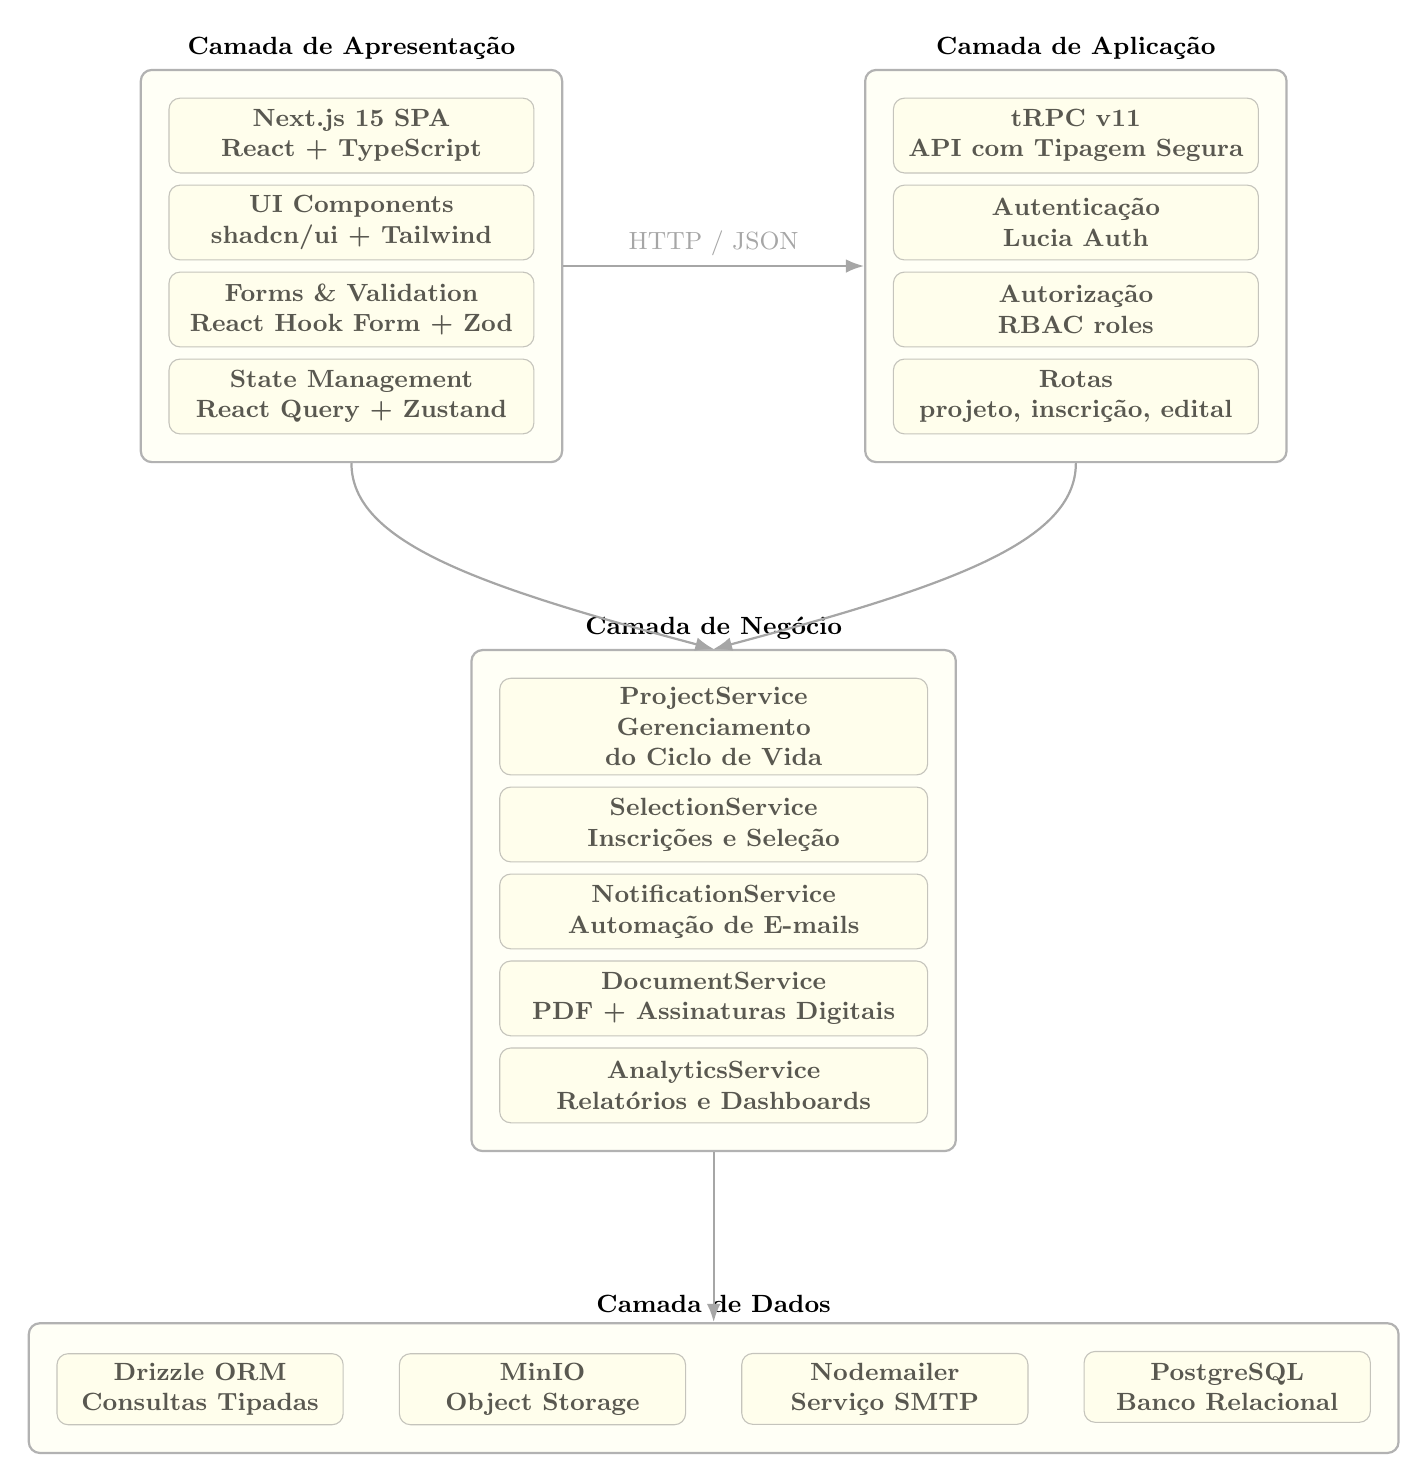
\begin{tikzpicture}[
    layer/.style={rounded corners, draw=gray!60, fill=yellow!10, fill opacity=0.35, draw opacity=1, thick, inner sep=10pt},
    box/.style={draw=gray!70, rounded corners, fill=yellow!6, text width=4.4cm, align=center, minimum height=0.95cm, font=\small\bfseries, text=black},
    smallbox/.style={draw=gray!70, rounded corners, fill=yellow!6, text width=5.2cm, align=center, minimum height=0.95cm, font=\small\bfseries, text=black},
    databox/.style={draw=gray!70, rounded corners, fill=yellow!6, text width=3.4cm, align=center, minimum height=0.9cm, font=\small\bfseries, text=black},
    connector/.style={-Latex, thick, gray!70}
  ]
    % Camada de Apresentação
    \matrix (presentation) [
      matrix of nodes,
      nodes={box},
      row sep=4pt,
      column sep=0pt,
      matrix anchor=north,
      anchor=north
    ] at (-4.6,0) {
      {Next.js 15 SPA\\React + TypeScript} \\
      {UI Components\\shadcn/ui + Tailwind} \\
      {Forms \& Validation\\React Hook Form + Zod} \\
      {State Management\\React Query + Zustand} \\
    };
    \node[layer, fit=(presentation-1-1)(presentation-4-1), label={[font=\small\bfseries]above:Camada de Apresentação}] (presentationLayer) {};

    % Camada de Aplicação
    \matrix (application) [
      matrix of nodes,
      nodes={box},
      row sep=4pt,
      column sep=0pt,
      matrix anchor=north,
      anchor=north
    ] at (4.6,0) {
      {tRPC v11\\API com Tipagem Segura} \\
      {Autenticação\\Lucia Auth} \\
      {Autorização\\RBAC roles} \\
      {Rotas\\projeto, inscrição, edital} \\
    };
    \node[layer, fit=(application-1-1)(application-4-1), label={[font=\small\bfseries]above:Camada de Aplicação}] (applicationLayer) {};

    % Camada de Negócio
    \coordinate (topMid) at ($(presentationLayer.south)!0.5!(applicationLayer.south)$);
    \matrix (business) [
      matrix of nodes,
      nodes={smallbox},
      row sep=4pt,
      column sep=0pt,
      matrix anchor=north,
      anchor=north
    ] at ($(topMid)+(0,-2.6)$) {
      {ProjectService\\Gerenciamento do Ciclo de Vida} \\
      {SelectionService\\Inscrições e Seleção} \\
      {NotificationService\\Automação de E-mails} \\
      {DocumentService\\PDF + Assinaturas Digitais} \\
      {AnalyticsService\\Relatórios e Dashboards} \\
    };
    \node[layer, fit=(business-1-1)(business-5-1), label={[font=\small\bfseries]above:Camada de Negócio}] (businessLayer) {};

    % Camada de Dados
    \matrix (data) [
      matrix of nodes,
      nodes={databox},
      row sep=0pt,
      column sep=0.7cm,
      matrix anchor=north,
      anchor=north
    ] at ($(businessLayer.south)+(0,-2.4)$) {
      {Drizzle ORM\\Consultas Tipadas} &
      {MinIO\\Object Storage} &
      {Nodemailer\\Serviço SMTP} &
      {PostgreSQL\\Banco Relacional} \\
    };
    \node[layer, fit=(data-1-1)(data-1-4), label={[font=\small\bfseries]above:Camada de Dados}] (dataLayer) {};

    % Conectores
    \draw[connector] (presentationLayer.east) -- node[above,font=\small]{HTTP / JSON} (applicationLayer.west);
    \draw[connector] (presentationLayer.south) .. controls +(0,-1.0) and +(-3,0.8) .. (businessLayer.north);
    \draw[connector] (applicationLayer.south) .. controls +(0,-1.0) and +(3,0.8) .. (businessLayer.north);
    \draw[connector] (businessLayer.south) -- (dataLayer.north);
  \end{tikzpicture}
  \caption{Arquitetura lógica do Sistema de Monitoria-IC.}
  \label{fig:architecture}
\end{figure}

\clearpage

A camada de apresentação foi implementada como uma Single Page Application (SPA) utilizando Next.js 15, React e TypeScript, proporcionando uma interface responsiva construída a partir de componentes shadcn/ui e Tailwind CSS. O roteamento é dinâmico e protegido por papéis, assegurando que cada perfil de usuário (administrador, professor ou estudante) tenha acesso apenas às funcionalidades pertinentes. O estado do cliente é coordenado por React Query, que gerencia cache e sincronização de dados remotos, e Zustand, que cuida do estado local da aplicação. Os formulários utilizam React Hook Form para gerenciamento eficiente de estado e validações, combinado com Zod para garantir consistência entre as validações de cliente e servidor.

O sistema oferece interfaces especializadas estruturadas em módulos funcionais para cada perfil de usuário. Para o perfil de administrador, são disponibilizados sete módulos principais que refletem as responsabilidades de coordenação do programa de monitoria. O módulo Dashboard consolida métricas operacionais e indicadores em tempo real, incluindo distribuição de projetos por status (rascunho, submetido, aprovado, rejeitado), número total de inscrições por período letivo e visualização rápida de prazos críticos. O módulo Projetos centraliza o gerenciamento completo do ciclo de vida de projetos de monitoria: visualização e aprovação de projetos submetidos pelos docentes, importação de planejamento semestral via planilha Excel com dados SIAPE (Sistema Integrado de Administração de Pessoal), e alocação de bolsas por projeto com validação automática de limites totais informados pela PROGRAD, impedindo excedentes. O módulo Editais permite criar, configurar e publicar editais internos do departamento, definindo datas de inscrição, pontos de prova e bibliografia, além de solicitar assinatura digital do chefe do departamento antes da publicação, com envio automatizado de notificações por e-mail. O módulo Documentos oferece gestão centralizada de arquivos, incluindo históricos acadêmicos, comprovantes de matrícula, documentos de identificação e PDFs gerados pelo sistema (projetos assinados, editais, atas), com suporte a versionamento e metadados para auditoria. O módulo Usuários implementa funcionalidades CRUD completas para administração de contas de professores e alunos, permitindo pesquisa avançada por nome, matrícula ou SIAPE, edição de perfis acadêmicos e envio de convites institucionais para novos docentes. O módulo Configurações abrange o cadastro e manutenção de cursos de graduação, departamentos acadêmicos, disciplinas com códigos oficiais, configuração de equivalências curriculares (fundamental para o processo seletivo que considera disciplinas equivalentes ao calcular notas), e parâmetros de integração SMTP para envio automatizado de notificações. Por fim, o módulo Sistema consolida funcionalidades analíticas e gerenciais: analytics com visualizações de tendências históricas (evolução de inscrições, distribuição de bolsas por departamento ao longo dos semestres), relatórios consolidados estruturados para PROGRAD (listagem de monitores ativos com dados de pagamento) e planilhas finais em formato Excel diferenciando bolsistas e voluntários, com links para PDFs dos projetos aprovados.

Para o perfil de professor, o sistema estrutura-se em quatro módulos que cobrem as responsabilidades docentes no programa de monitoria. O módulo Meus Projetos permite criar, editar e gerenciar projetos individuais ou coletivos (quando múltiplos professores ministram uma mesma disciplina), com funcionalidade de reutilização de templates de semestres anteriores para agilizar a criação, edição de título, descrição, atividades e carga horária, e assinatura digital com visualização prévia do PDF antes da submissão administrativa. O módulo Processo Seletivo concentra todas as etapas relacionadas à seleção de monitores: gerenciar candidatos permite visualizar lista de alunos inscritos em cada projeto com informações acadêmicas (CR, nota na disciplina considerando equivalências configuradas), documentos anexados (histórico, comprovante de matrícula) e tipo de vaga pretendida (bolsista, voluntário ou ambos); avaliar candidatos oferece interface para atribuição de notas de prova e entrevista, com cálculo automático da nota final ponderada conforme critérios institucionais; selecionar monitores apresenta lista ranqueada de candidatos por nota final, permitindo escolha de bolsistas até o limite alocado pela administração e definição de voluntários até o limite configurado pelo próprio professor; e publicar resultados gera automaticamente atas de seleção em PDF e dispara notificações por e-mail para todos os candidatos, informando aprovação (bolsista ou voluntário), lista de espera ou não seleção. O módulo Documentos permite gerar e assinar atas de seleção (documento oficial registrando o processo seletivo, critérios utilizados, candidatos inscritos e resultado final) e termos de compromisso (documento assinado digitalmente pelo professor e pelo monitor, estabelecendo responsabilidades, carga horária e atividades previstas). Por fim, o módulo Gestão Acadêmica oferece configuração e acompanhamento de monitores voluntários adicionais além dos definidos no edital, permitindo que o professor amplie sua equipe de monitoria conforme demanda da disciplina, embora sem remuneração institucional.

Para o perfil de estudante, o sistema disponibiliza um módulo unificado de Monitoria com quatro funcionalidades principais que cobrem a jornada completa do aluno. A funcionalidade Inscrição em Monitoria permite que o estudante se inscreva em projetos disponíveis no período ativo de inscrições, informando preferência por vaga bolsista, voluntária ou ambas, com upload obrigatório de histórico acadêmico atualizado, comprovante de matrícula vigente e documento de identificação. A funcionalidade Vagas Disponíveis apresenta catálogo paginado de projetos com vagas abertas, com filtros por departamento acadêmico (DCC, DCI), tipo de vaga (bolsista, voluntário) e busca textual por título de disciplina ou nome do professor orientador, exibindo para cada projeto: nome da disciplina, código oficial, professores responsáveis, número de vagas bolsistas e voluntárias disponíveis, carga horária semanal e descrição das atividades previstas. A funcionalidade Resultados das Seleções exibe lista de todas as inscrições realizadas pelo aluno no período letivo atual, indicando para cada uma o status detalhado (selecionado bolsista, selecionado voluntário, lista de espera com posição, ou não selecionado), com resumo agregado por categoria no topo da página e notificações automáticas quando novos resultados são publicados pelos professores. Por fim, a funcionalidade Meu Status consolida informações de aceite ou rejeição de vagas oferecidas, com formulário para preenchimento de dados bancários quando o aluno aceita uma vaga bolsista (banco, agência, número da conta e dígito verificador), além de indicadores visuais de pendências que possam impedir a efetivação da monitoria (dados bancários incompletos, documentação faltante ou termo de compromisso não assinado).

A camada de aplicação utiliza tRPC v11 para prover uma API completamente \textit{type-safe} entre cliente e servidor, eliminando a necessidade de definições duplicadas de tipos e reduzindo significativamente a possibilidade de erros de integração. As procedures são organizadas por domínio (projeto, inscrição, edital, entre outros), facilitando a manutenção e evolução do sistema. A autenticação é realizada via Lucia Auth, um framework moderno e seguro que gerencia sessões de usuário com duração configurável de 30 dias. As validações ocorrem automaticamente em ambos os lados da comunicação através de esquemas Zod compartilhados, e o sistema oferece suporte a \textit{subscriptions} para atualizações em tempo quase real, permitindo que múltiplos usuários visualizem mudanças de estado instantaneamente.

A camada de negócio concentra a lógica central do sistema em serviços especializados e desacoplados. O \texttt{ProjectService} gerencia o ciclo de vida completo de projetos de monitoria, desde a criação com base em templates até a consolidação final para PROGRAD. O \texttt{SelectionService} processa as inscrições de estudantes e executa a lógica de seleção, considerando critérios como coeficiente de rendimento, nota na disciplina e equivalências curriculares. O \texttt{NotificationService} orquestra o envio de notificações por e-mail em todas as etapas do processo, garantindo que professores, estudantes e administradores sejam informados sobre mudanças de estado relevantes. O \texttt{DocumentService} é responsável pela geração de documentos PDF (projetos, editais, relatórios) e pelo gerenciamento de assinaturas digitais, tanto dos professores quanto do chefe do departamento. Por fim, o \texttt{AnalyticsService} consolida dados transacionais em métricas e indicadores apresentados nos dashboards administrativos, fornecendo visões agregadas do processo de monitoria para apoiar a tomada de decisões institucionais.

A camada de dados utiliza PostgreSQL como sistema gerenciador de banco de dados relacional, combinado com Drizzle ORM para garantir consultas tipadas e seguras. O esquema de dados foi normalizado seguindo as formas normais clássicas, mantendo integridade referencial entre todas as entidades do domínio. As migrações são versionadas e reversíveis, permitindo evolução controlada do modelo de dados ao longo do tempo. Índices foram criados estrategicamente nas colunas mais consultadas para otimizar o desempenho de queries frequentes, especialmente aquelas relacionadas à listagem de projetos por período, busca de inscrições por estudante e geração de relatórios consolidados. Para armazenamento de arquivos (históricos acadêmicos, documentos comprobatórios, PDFs gerados), o sistema utiliza MinIO, uma solução compatível com o protocolo S3 que oferece escalabilidade horizontal e facilita futuras migrações para serviços de nuvem. Rotinas automatizadas de backup incremental são executadas a cada seis horas, com retenção de 30 dias, assegurando resiliência e possibilidade de recuperação em caso de falhas.

Além dos aspectos funcionais e arquiteturais, o Sistema de Monitoria-IC foi concebido considerando requisitos de segurança da informação e privacidade de dados, em consonância com a Lei Geral de Proteção de Dados (LGPD). A autenticação é realizada por meio de Lucia Auth, com sessões protegidas e gerenciamento explícito de papéis (administração, professor, estudante), implementando um modelo de controle de acesso baseado em papéis (RBAC, do inglês \textit{Role-Based Access Control}) que restringe o acesso a dados e funcionalidades de acordo com o perfil do usuário. O uso de um ORM tipado (Drizzle) contribui para mitigar riscos de injeção de SQL, enquanto a comunicação cliente-servidor é projetada para operar sobre HTTPS em ambiente de produção, assegurando a confidencialidade dos dados em trânsito. Do ponto de vista de privacidade, o sistema adota o princípio da minimização de dados, armazenando apenas informações pessoais estritamente necessárias para a gestão da monitoria (por exemplo, identificação do aluno, histórico acadêmico relevante e dados bancários de bolsistas). Políticas de retenção de dados e de acesso a relatórios podem ser configuradas para atender às diretrizes institucionais, e o histórico de operações mantém trilhas de auditoria para fins de transparência e responsabilização. A interface Web foi desenvolvida com responsividade, visando funcionamento adequado em diferentes tamanhos de tela (desktop, tablet e dispositivos móveis) e utilizando componentes que suportam navegação por teclado. Embora uma avaliação formal de acessibilidade ainda não tenha sido conduzida, o sistema segue boas práticas básicas de design de interface (uso consistente de hierarquia visual, contrastes adequados e feedback claro de ações), abrindo caminho para evoluções futuras em direção à conformidade com as diretrizes WCAG 2.1 em nível institucional.

\subsection{Modelo de Dados}

O modelo de dados foi projetado para capturar todas as entidades e relacionamentos do domínio de monitoria, seguindo princípios de normalização e integridade referencial. A Figura \ref{fig:data-model} apresenta as principais entidades e seus relacionamentos:

\clearpage

\begin{figure}[p]
  \centering
  \includegraphics[width=0.95\textwidth,keepaspectratio]{images/monitoria/data-model-erd.png}
  \caption{Modelo de dados resumido do domínio de monitoria.}
  \label{fig:data-model}
\end{figure}

\clearpage

O dashboard administrativo consolida indicadores operacionais (projetos por status, períodos de inscrição, volume de candidaturas) e oferece navegação rápida para tarefas críticas do papel \textit{admin}, conforme a estrutura do menu lateral.

No núcleo de usuários, a entidade \texttt{user} concentra autenticação e perfil básico, estendida por perfis específicos de \texttt{professor} (dados acadêmicos) e \texttt{aluno} (matrícula, curso e CR), com papéis representados por \texttt{role} (\textit{admin}, \textit{professor}, \textit{student}). No eixo acadêmico, \texttt{departamento}, \texttt{curso} e \texttt{disciplina} descrevem a hierarquia institucional, os cursos vinculados e as disciplinas (com códigos e equivalências). No domínio da monitoria, \texttt{periodo\_inscricao} e \texttt{edital} organizam publicações por semestre; \texttt{projeto} evolui por estados bem definidos (DRAFT, SUBMITTED, APPROVED/REJECTED) e se relaciona a \texttt{projeto\_template} para reuso; \texttt{inscricao} registra candidaturas e notas; \texttt{vaga} modela posições de monitor (BOLSISTA, VOLUNTARIO); e \texttt{importacao\_planejamento} registra o histórico de importações semestrais (com arquivo, totalizações e usuário responsável).

\subsection{Fluxo de Processos}

O fluxo de monitoria é orquestrado em cinco etapas contínuas que estruturam o semestre, conforme ilustrado na Figura \ref{fig:process-flow}. Neste trabalho, a etapa enfatizada (e adotada como foco da validação do sistema) é o fluxo de \textit{Planejamento \& Criação} até \textit{Aprovação \& PROGRAD}, pois concentra o maior impacto na redução de retrabalho e na padronização dos documentos encaminhados ao Instituto. Na prática, esse fluxo se materializa em módulos específicos da aplicação: (i) a administração acessa \textit{Importar Planejamento} para enviar a planilha semestral; o sistema valida o arquivo, cria projetos iniciais por disciplina e dispara notificações automáticas aos professores, sinalizando que há projetos pendentes de revisão e assinatura; (ii) ao acessar o dashboard, o professor visualiza os projetos em estado de pendência e, caso não exista template prévio, é conduzido a criar um template padrão da disciplina (título, descrição, carga horária e atividades), permitindo reuso nos próximos semestres; (iii) em seguida, o professor revisa o projeto do semestre, gera o PDF e realiza a assinatura digital no módulo \textit{Assinatura de Documentos}; (iv) a submissão assinada torna o projeto elegível para revisão administrativa em \textit{Gerenciar Projetos}, onde o administrador pode aprovar ou rejeitar com feedback; e (v) quando aprovado, o projeto passa a compor automaticamente a planilha consolidada em \textit{Planilha para Instituto}, disponível para download e envio por e-mail, incluindo referências e anexos aos PDFs dos projetos aprovados, facilitando o trâmite com o Instituto/PROGRAD.

As demais etapas (\textit{Alocação \& Edital}, \textit{Inscrições \& Seleção} e \textit{Aceite \& Consolidação}) complementam o ciclo e já estão contempladas no sistema, permitindo a configuração de vagas, publicação de edital interno, inscrição de estudantes, seleção e consolidação final de dados bancários e planilhas para órgãos responsáveis.\footnote{O recorte deste trabalho segue o planejamento visível na Figura 3, com foco nas fases implementadas até a geração da planilha consolidada para o Instituto/PROGRAD. Esse fluxo foi revisado passo a passo em conjunto com o Prof.\ Rubisley de Paula Lemes, assegurando aderência ao procedimento esperado no contexto do Instituto de Computação.}

\begin{figure}[htb]
  \centering
  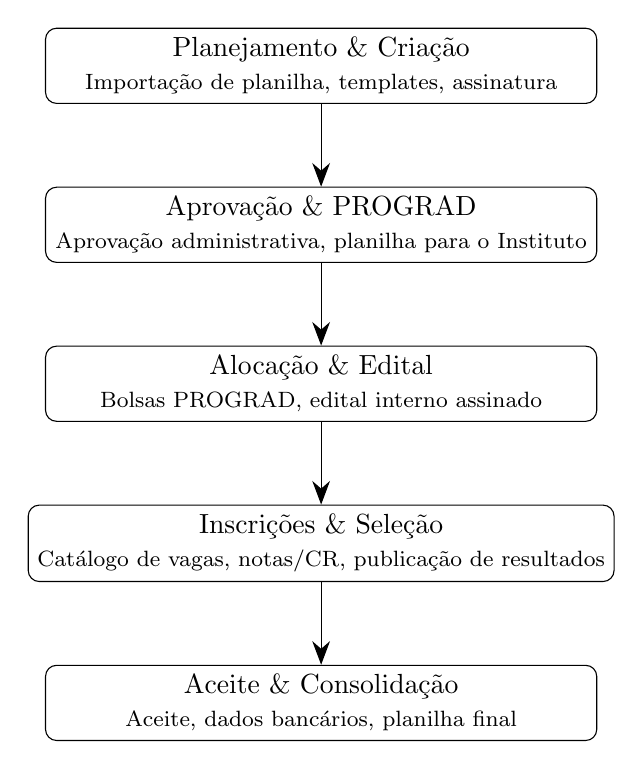
\begin{tikzpicture}[
    node distance=1.05cm,
    every node/.style={rounded corners, draw, align=center, minimum width=7cm, minimum height=0.82cm},
    >={Stealth[length=3mm]}
  ]
    \node (fase1) {Planejamento \& Criação\\\footnotesize Importação de planilha, templates, assinatura};
    \node[below=of fase1] (fase2) {Aprovação \& PROGRAD\\\footnotesize Aprovação administrativa, planilha para o Instituto};
    \node[below=of fase2] (fase3) {Alocação \& Edital\\\footnotesize Bolsas PROGRAD, edital interno assinado};
    \node[below=of fase3] (fase4) {Inscrições \& Seleção\\\footnotesize Catálogo de vagas, notas/CR, publicação de resultados};
    \node[below=of fase4] (fase5) {Aceite \& Consolidação\\\footnotesize Aceite, dados bancários, planilha final};

    \draw[->] (fase1) -- (fase2);
    \draw[->] (fase2) -- (fase3);
    \draw[->] (fase3) -- (fase4);
    \draw[->] (fase4) -- (fase5);
  \end{tikzpicture}
  \caption{Fluxo de processos do semestre de monitoria.}
  \label{fig:process-flow}
\end{figure}

Em \textit{Gerenciar Projetos}, o administrador acompanha submissões, aprovações e gera a planilha consolidada para o Instituto/PROGRAD, garantindo padronização e trilhas de auditoria.

\subsection{Implementação e Tecnologias}

O sistema foi implementado utilizando um conjunto coeso de tecnologias modernas e consolidadas, selecionadas para maximizar produtividade de desenvolvimento, segurança e manutenibilidade. No \textit{frontend}, adotou-se Next.js 15.1.4 com App Router, um framework React de produção que oferece renderização híbrida (SSR e CSR), otimizações automáticas de desempenho e roteamento baseado em sistema de arquivos. TypeScript 5.x foi utilizado em todo o código-fonte para garantir \textit{type safety} e detectar erros em tempo de desenvolvimento. A interface visual foi construída com Tailwind CSS, um framework utilitário que proporciona consistência e rapidez na estilização, complementado por shadcn/ui, uma coleção de componentes acessíveis e personalizáveis. Os formulários são implementados com React Hook Form, que minimiza re-renderizações desnecessárias e oferece validação eficiente, combinado com Zod para esquemas de validação compartilhados entre cliente e servidor. A sincronização de estado remoto e o gerenciamento de cache são tratados por React Query (TanStack Query), que automatiza requisições, invalidações e atualizações otimistas.

No \textit{backend}, a API foi construída com tRPC v11, uma solução inovadora que elimina a necessidade de definições duplicadas de tipos entre cliente e servidor, garantindo que toda comunicação seja completamente tipada em tempo de compilação. A autenticação e gerenciamento de sessões são realizados por Lucia Auth, um framework moderno que oferece flexibilidade e segurança superiores a soluções legadas. A persistência de dados utiliza Drizzle ORM em conjunto com PostgreSQL, proporcionando consultas SQL tipadas e migrações versionadas de forma declarativa. Para armazenamento de arquivos binários (históricos acadêmicos, documentos comprobatórios, PDFs gerados), o sistema emprega MinIO, uma solução compatível com o protocolo S3 da Amazon que facilita futuras migrações para serviços de nuvem. O envio automatizado de notificações por e-mail é realizado via Nodemailer, configurado para utilizar o servidor SMTP institucional da UFBA.

A infraestrutura de \textit{DevOps} foi projetada para garantir qualidade e confiabilidade através de práticas modernas de integração e entrega contínuas. A solução completa é containerizada com Docker, incluindo o banco de dados PostgreSQL, o servidor MinIO e a aplicação Node.js, facilitando implantação consistente em diferentes ambientes (desenvolvimento, homologação e produção). Uma pipeline automatizada no GitHub Actions executa validações a cada commit: linting e formatação de código com Biome, verificação estática de tipos com TypeScript, execução de testes unitários com Vitest para validar a lógica de negócio, execução de testes end-to-end com Playwright para validar fluxos completos do usuário, e build de produção para detectar erros de compilação antecipadamente. Essa abordagem garante que apenas código validado e livre de regressões seja promovido para ambientes de produção.

A organização da lógica de negócio segue uma estrutura modular baseada em routers tRPC especializados por domínio. O router principal (\texttt{appRouter}) agrega routers específicos para autenticação e usuários (\texttt{auth}, \texttt{me}, \texttt{user}, \texttt{apiKey}), entidades acadêmicas (\texttt{departamento}, \texttt{curso}, \texttt{discipline}), gestão de monitoria (\texttt{projeto}, \texttt{projetoTemplates}, \texttt{edital}, \texttt{inscricao}, \texttt{selecao}, \texttt{vagas}), funcionalidades administrativas (\texttt{importProjects}, \texttt{scholarshipAllocation}, \texttt{analytics}, \texttt{relatorios}) e infraestrutura transversal (\texttt{file}, \texttt{signature}, \texttt{notificacoes}). Essa separação facilita a compreensão do código, permite testes isolados de cada módulo e viabiliza o desenvolvimento paralelo por múltiplos desenvolvedores sem conflitos significativos.

\subsection{Interfaces do Sistema}

O sistema oferece interfaces especializadas para cada perfil de usuário, conforme exemplificado nas Figuras \ref{fig:landing} a \ref{fig:admin-departamentos}. A página inicial (Figura \ref{fig:landing}) apresenta a proposta do sistema, acesso ao login institucional e comunicação de períodos de inscrição quando ativos, funcionando como ponto de entrada para estudantes, professores e administradores. A tela de login (Figura \ref{fig:login}) valida credenciais locais ou redireciona ao CAS quando habilitado, estabelecendo a sessão do usuário e direcionando ao dashboard apropriado.

\begin{figure}[h!]
  \centering
  \includegraphics[width=\linewidth]{images/monitoria/landing.png}
  \caption{Página inicial pública do sistema.}
  \label{fig:landing}
\end{figure}

\begin{figure}[h!]
  \centering
  \includegraphics[width=\linewidth]{images/monitoria/login.png}
  \caption{Tela de login local do sistema.}
  \label{fig:login}
\end{figure}

O dashboard administrativo (Figura \ref{fig:dashboard}) consolida indicadores operacionais (projetos por status, períodos de inscrição, volume de candidaturas) e oferece navegação rápida para tarefas críticas do papel \textit{admin}. A interface de assinatura de projetos (Figura \ref{fig:professor-assinatura}) permite que o professor visualize o PDF gerado, use a assinatura padrão do perfil ou desenhe uma nova assinatura antes de submeter para análise administrativa.

\begin{figure}[h!]
  \centering
  \includegraphics[width=\linewidth]{images/monitoria/admin-dashboard.png}
  \caption{Dashboard administrativo com métricas.}
  \label{fig:dashboard}
\end{figure}

\begin{figure}[h!]
  \centering
  \includegraphics[width=\linewidth]{images/monitoria/professor-assinatura-documentos.png}
  \caption{Assinatura de projeto pelo professor.}
  \label{fig:professor-assinatura}
\end{figure}

Para estudantes, a tela de inscrição (Figura \ref{fig:student-inscricao}) oferece filtros por departamento e tipo de vaga, busca por título/professor e exibe avisos sobre o período ativo; quando o período está fechado, os componentes permanecem acessíveis para consulta e planejamento. A tela de resultados (Figura \ref{fig:student-resultados}) permite que o aluno acompanhe o status de cada inscrição (selecionado bolsista/voluntário, lista de espera, não selecionado) e o resumo agregado por categoria.

\begin{figure}[h!]
  \centering
  \includegraphics[width=\linewidth]{images/monitoria/student-inscricao-monitoria.png}
  \caption{Inscrição do aluno em projetos de monitoria.}
  \label{fig:student-inscricao}
\end{figure}

\begin{figure}[h!]
  \centering
  \includegraphics[width=\linewidth]{images/monitoria/student-resultados.png}
  \caption{Resultados das seleções para o aluno.}
  \label{fig:student-resultados}
\end{figure}

As funcionalidades administrativas incluem o gerenciamento de projetos (Figura \ref{fig:projetos}), onde o administrador acompanha submissões e aprovações e gera a planilha consolidada para o Instituto/PROGRAD; a gestão de editais (Figura \ref{fig:editais}), que permite configurar datas, pontos de prova e bibliografia, solicitar assinatura digital do chefe do departamento e publicar com notificações automáticas; e a alocação de bolsas (Figura \ref{fig:bolsas}), que impede excedentes em relação ao total de bolsas concedidas pela PROGRAD.

\begin{figure}[h!]
  \centering
  \includegraphics[width=\linewidth]{images/monitoria/admin-manage-projects.png}
  \caption{Gerenciamento de projetos por semestre.}
  \label{fig:projetos}
\end{figure}

\begin{figure}[h!]
  \centering
  \includegraphics[width=\linewidth]{images/monitoria/admin-edital-management.png}
  \caption{Gestão de editais com status e ações.}
  \label{fig:editais}
\end{figure}

\begin{figure}[h!]
  \centering
  \includegraphics[width=\linewidth]{images/monitoria/admin-scholarship-allocation.png}
  \caption{Interface de alocação de bolsas.}
  \label{fig:bolsas}
\end{figure}

Completam as interfaces administrativas a gestão de usuários (Figura \ref{fig:admin-users}), onde a administração pesquisa, filtra e gerencia contas mantendo coerência com regras institucionais; a importação de planejamento (Figura \ref{fig:admin-import}), que processa planilhas do planejamento e emite relatório de inconsistências; e a tela de departamentos (Figura \ref{fig:admin-departamentos}), que permite manter a estrutura acadêmica essencial para vínculos de disciplinas e projetos. Por fim, a geração da planilha para a PROGRAD (Figura \ref{fig:planilha-prograd}) consolida todos os projetos aprovados em formato exportável para envio ao Instituto.

\begin{figure}[h!]
  \centering
  \includegraphics[width=\linewidth]{images/monitoria/admin-users.png}
  \caption{Administração de usuários.}
  \label{fig:admin-users}
\end{figure}

\begin{figure}[h!]
  \centering
  \includegraphics[width=\linewidth]{images/monitoria/admin-import-projects.png}
  \caption{Importação de planejamento.}
  \label{fig:admin-import}
\end{figure}

\begin{figure}[h!]
  \centering
  \includegraphics[width=\linewidth]{images/monitoria/admin-departamentos.png}
  \caption{Gestão de departamentos.}
  \label{fig:admin-departamentos}
\end{figure}

\begin{figure}[h!]
  \centering
  \includegraphics[width=\linewidth]{images/monitoria/admin-planilha-prograd.png}
  \caption{Geração de planilha PROGRAD com projetos aprovados.}
  \label{fig:planilha-prograd}
\end{figure}

\section{Avaliação Experimental}
\label{sec:evaluation}

O objetivo desta avaliação experimental é validar a efetividade do Sistema de Monitoria-IC em dois eixos complementares: (i) eficiência operacional, mensurando ganhos potenciais em tempo, redução de erros e automação de tarefas em relação ao processo manual anterior; e (ii) qualidade técnica da implementação, analisando robustez, cobertura de testes e aderência da arquitetura às boas práticas de sistemas de informação. Nesta seção, descrevem-se a metodologia adotada, os resultados técnicos obtidos e as principais limitações e ameaças à validade.

\subsection{Metodologia}

A avaliação foi conduzida em ambiente de desenvolvimento e teste, utilizando dados de exemplo que reproduzem cenários reais de monitoria do Instituto de Computação. A metodologia adotada combinou três frentes principais:

\begin{enumerate}
  \item Testes end-to-end (E2E): foram especificados cenários automatizados que percorrem o fluxo completo de monitoria, desde a criação e submissão de projetos pelos docentes até a seleção de monitores, aceite de vagas e consolidação final para a PROGRAD. Esses cenários incluem variações de papéis (administração, professores, estudantes), estados de projetos (rascunho, submetido, aprovado) e tipos de vaga (bolsista, voluntário).

  \item Testes unitários e de integração: serviços centrais da camada de negócio (gestão de projetos, inscrições, seleção, relatórios) foram exercitados por meio de testes unitários e de integração, verificando regras de negócio críticas, validações de dados e interações com a camada de dados. A utilização de um ORM tipado (Drizzle) facilitou a detecção de inconsistências entre modelo de dados e código.

  \item Métricas de execução e logs de aplicação: durante a execução dos testes automatizados, foram coletadas métricas de tempo de resposta das principais rotas e registros de log para monitorar possíveis falhas, exceções não tratadas ou degradação de desempenho. Essas informações subsidiam a análise de robustez e escalabilidade da solução em cenários típicos de uso.
\end{enumerate}

Não foi realizado, até o momento, um piloto formal em produção com usuários finais (docentes, estudantes e administradores). A avaliação com pessoas usuárias é, portanto, considerada trabalho futuro, a ser conduzida em ambiente real de monitoria, conforme discutido na Seção~\ref{sec:conclusion}.

\subsection{Resultados Técnicos}

Os resultados obtidos até esta etapa de avaliação concentram-se na dimensão técnica do sistema. A Tabela~\ref{tab:resultados-tecnicos} sintetiza alguns indicadores relevantes dos testes automatizados executados.

\begin{table}[htb]
  \centering
  \small
  \caption{Síntese de resultados técnicos da avaliação preliminar.}
  \label{tab:resultados-tecnicos}
  \begin{tblr}{
    width=\linewidth,
    colspec={|Q[l,2.5cm]|X[l]|},
    hlines,
    vlines
  }
    \textbf{Indicador} & \textbf{Valor Medido} \\
    Testes unitários & 57 testes em 16 arquivos, cobrindo routers tRPC (autenticação, projetos, inscrições, seleção, editais, arquivos, analytics) \\
    Taxa de sucesso & 100\% (57/57 testes aprovados sem falhas ou regressões) \\
    Tempo execução & 1.07s para a suíte completa (73ms em testes, 173ms em setup, 992ms em transformação TypeScript) \\
    Inicialização & Servidor Next.js iniciando em 1.34s em ambiente de desenvolvimento \\
    Cobertura funcional & Validação de regras críticas: controle de acesso RBAC, workflow de projetos, processo seletivo, importação de planejamento, publicação de editais \\
    Estabilidade & Zero erros críticos não tratados; todas as exceções de negócio corretamente transformadas em TRPCError \\
  \end{tblr}
\end{table}

A execução dos testes unitários e de integração demonstrou robustez na implementação das regras de negócio e validações de autorização. Os 57 testes automatizados, distribuídos em 16 arquivos de teste organizados por domínio (departamento, curso, disciplina, projeto, inscrição, edital, seleção, usuário, arquivo, termos, analytics), cobrem fluxos críticos do sistema: controle de acesso baseado em papéis (verificando que administradores, professores e estudantes acessam apenas funcionalidades pertinentes), workflow de aprovação de projetos (transições de estado DRAFT → SUBMITTED → APPROVED/REJECTED), processo seletivo com cálculo automático de notas finais ponderadas, importação de planejamento com validação de consistência de dados SIAPE, publicação de editais com validação de assinatura digital obrigatória, e gerenciamento de inscrições considerando equivalências curriculares configuradas. A taxa de sucesso de 100\% e o tempo de execução reduzido (1.07s para toda a suíte) evidenciam a estabilidade da solução e a eficácia das práticas de desenvolvimento adotadas, incluindo validação estática de tipos via TypeScript, uso de ORM tipado (Drizzle) para prevenir inconsistências entre modelo de dados e código, e pipeline de integração contínua executando testes automaticamente a cada commit.

As métricas de desempenho coletadas em ambiente de desenvolvimento local indicam tempo de inicialização do servidor Next.js de 1.34 segundos, demonstrando otimização adequada do processo de build e carregamento de dependências. A arquitetura adotada, com separação clara entre camadas de apresentação, aplicação, negócio e dados, contribui para a manutenibilidade e testabilidade do sistema, permitindo validação isolada de cada componente e facilitando a identificação de regressões. A utilização de tRPC v11 para comunicação type-safe entre cliente e servidor elimina categorias inteiras de erros de integração, conforme evidenciado pela ausência de falhas relacionadas a incompatibilidades de tipos ou contratos de API nos testes executados.

Cabe ressaltar que esta avaliação concentra-se em aspectos técnicos e funcionais do sistema, validando a corretude da implementação em relação aos requisitos especificados na Tabela~\ref{tab:requisitos}. Uma avaliação complementar com usuários finais (professores, estudantes e administradores) em ambiente real de monitoria, incluindo métricas de usabilidade percebida, satisfação, curva de aprendizado e impacto efetivo na redução de tempo gasto em tarefas administrativas, permanece como trabalho futuro prioritário, conforme discutido na Seção~\ref{sec:conclusion}.

\subsection{Avaliação com Professores (Validação Preliminar)}

Além da validação técnica descrita acima, foi conduzida uma avaliação preliminar com docentes, com foco no fluxo enfatizado neste trabalho (importação de planejamento \(\rightarrow\) criação/reuso de templates \(\rightarrow\) assinatura de projetos \(\rightarrow\) aprovação administrativa \(\rightarrow\) geração de planilha para o Instituto/PROGRAD). A pesquisa foi aplicada apenas com professores por duas razões: (i) o papel \textit{admin} é tipicamente representado por um conjunto reduzido de usuários (1--2), e (ii) os docentes apresentam maior diversidade de perfil e uso ao longo do processo, oferecendo evidências mais ricas para análise inicial.

Como validação qualitativa do fluxo, o passo-a-passo foi revisado e conferido em conjunto com o Prof.\ Rubisley de Paula Lemes, verificando a aderência do sistema às etapas administrativas e às ações esperadas do professor no ciclo de criação e submissão do projeto.

Para capturar percepção de utilidade e satisfação, foi aplicado um questionário estruturado, composto por 10 questões em escala Likert (1 a 5) e 2 questões de resposta binária (Sim/Não). As Tabelas~\ref{tab:questionario-professores} e~\ref{tab:questionario-professores-cont} apresentam o instrumento aplicado. Os valores numéricos e estatísticas apresentadas nas Tabelas~\ref{tab:avaliacao-professores-likert} e~\ref{tab:avaliacao-professores-binario} serão atualizados após a consolidação final das respostas.

A construção do instrumento foi orientada pelo fluxo end-to-end priorizado nesta monografia, de modo que cada pergunta estivesse diretamente associada a uma etapa do processo: notificação após importação do planejamento, criação e reuso de template por disciplina, geração e pré-visualização do PDF, assinatura e submissão do projeto, feedback administrativo e consolidação em planilha para o Instituto/PROGRAD. Dessa forma, buscou-se reduzir ambiguidade na interpretação e favorecer respostas ancoradas em funcionalidades concretas do sistema.

O questionário foi aplicado após uma demonstração guiada do fluxo e exploração livre do sistema pelos participantes. Para as questões Q1--Q10, utilizou-se escala Likert de 1 a 5, onde (1) \textit{Discordo totalmente}, (2) \textit{Discordo parcialmente}, (3) \textit{Neutro}, (4) \textit{Concordo parcialmente} e (5) \textit{Concordo totalmente}. As questões Q11--Q12 foram incluídas como indicadores binários de intenção de adoção e recomendação, complementando a avaliação de satisfação.

Na análise, as respostas serão consolidadas por distribuição de frequências e estatísticas descritivas (média, desvio padrão e variância) para as questões em escala, além da proporção de respostas Sim/Não nas questões binárias. Os resultados quantitativos serão preenchidos nesta seção após a coleta final do formulário (\textit{N} de respondentes e valores nas tabelas estão marcados como \textit{TODO}).

\begin{table*}[htb]
  \centering
  \small
  \caption{Questionário aplicado aos professores (enunciados completos).}
  \label{tab:questionario-professores}
  \begin{adjustbox}{max width=\textwidth}
    \begin{tblr}{
      width=\textwidth,
      colspec={|Q[c,1.2cm]|X[l]|},
      hlines,
      vlines
    }
      \textbf{Variável} & \textbf{Questão} \\
      Q1 & Após o administrador importar o planejamento semestral, o sistema identifica disciplinas e professores e notifica automaticamente o docente sobre projetos pendentes de revisão. Essa funcionalidade atendeu às suas expectativas? \\
      Q2 & Ao criar um projeto para uma disciplina, o sistema permite criar/atualizar um template padrão (título, descrição, carga horária, público-alvo e atividades) para reuso em semestres futuros. Essa funcionalidade atendeu às suas expectativas? \\
      Q3 & Ao reutilizar o template padrão, o preenchimento do projeto do semestre (com possibilidade de ajustes) reduz retrabalho e acelera a submissão do documento. Essa funcionalidade atendeu às suas expectativas? \\
      Q4 & A geração e pré-visualização do PDF do projeto antes da assinatura ajudam a reduzir erros e aumentam a confiança na submissão. Essa funcionalidade atendeu às suas expectativas? \\
      Q5 & O processo de assinatura digital do projeto no módulo \textit{Assinatura de Documentos} (abrir documento, assinar, submeter para análise) é simples e adequado para o fluxo do semestre. Como você avalia essa funcionalidade? \\
      Q6 & Após a assinatura e submissão, o feedback administrativo (aprovação/rejeição) é apresentado de forma clara e orienta correções quando necessário. Como você avalia essa funcionalidade? \\
    \end{tblr}
  \end{adjustbox}
\end{table*}

\begin{table*}[htb]
  \centering
  \small
  \caption{Continuação do questionário aplicado aos professores.}
  \label{tab:questionario-professores-cont}
  \begin{adjustbox}{max width=\textwidth}
    \begin{tblr}{
      width=\textwidth,
      colspec={|Q[c,1.2cm]|X[l]|},
      hlines,
      vlines
    }
      \textbf{Variável} & \textbf{Questão} \\
      Q7 & Os estados do projeto (por exemplo: rascunho, pendente de assinatura, em análise, aprovado, rejeitado) são compreensíveis e ajudam no acompanhamento do processo. Essa funcionalidade atendeu às suas expectativas? \\
      Q8 & A consolidação dos projetos aprovados em planilha para envio ao Instituto/PROGRAD (incluindo links/anexos para PDFs) facilita o trâmite administrativo do semestre. Essa funcionalidade atendeu às suas expectativas? \\
      Q9 & O fluxo implementado aumenta transparência e rastreabilidade das ações (quem fez o quê e em que etapa) no processo de monitoria. Essa funcionalidade atendeu às suas expectativas? \\
      Q10 & Considerando as fases 1 e 2 (importação, template, criação/assinatura e aprovação/planilha), qual o seu nível de satisfação geral com o Sistema de Monitoria-IC? \\
      Q11 & Você utilizaria o Sistema de Monitoria-IC no lugar do processo manual atual do Instituto de Computação? (Sim/Não) \\
      Q12 & Você recomendaria a adoção do Sistema de Monitoria-IC para o Instituto de Computação em um semestre de monitoria real? (Sim/Não) \\
    \end{tblr}
  \end{adjustbox}
\end{table*}

\begin{table*}[htb]
  \centering
  \small
  \caption{Distribuição das respostas (Likert 1--5) do questionário aplicado a professores.}
  \label{tab:avaliacao-professores-likert}
  \begin{adjustbox}{max width=\textwidth}
    \begin{tblr}{
      width=\textwidth,
      colspec={|Q[c,0.8cm]|Q[c,1.6cm]|X[l]|Q[c,0.55cm]|Q[c,0.55cm]|Q[c,0.55cm]|Q[c,0.55cm]|Q[c,0.55cm]|Q[c,1.0cm]|Q[c,1.2cm]|Q[c,1.2cm]|},
      hlines,
      vlines
    }
      \textbf{Q} & \textbf{Fator avaliado} & \textbf{Funcionalidade (resumo)} & \textbf{1} & \textbf{2} & \textbf{3} & \textbf{4} & \textbf{5} & \textbf{Média} & \textbf{Std. Desvio} & \textbf{Variância} \\
      Q1 & Expectativa & Importação e notificação automática após o planejamento. & \textit{TODO} & \textit{TODO} & \textit{TODO} & \textit{TODO} & \textit{TODO} & \textit{TODO} & \textit{TODO} & \textit{TODO} \\
      Q2 & Expectativa & Criação/edição de template padrão por disciplina. & \textit{TODO} & \textit{TODO} & \textit{TODO} & \textit{TODO} & \textit{TODO} & \textit{TODO} & \textit{TODO} & \textit{TODO} \\
      Q3 & Expectativa & Reuso do template no projeto do semestre (redução de retrabalho). & \textit{TODO} & \textit{TODO} & \textit{TODO} & \textit{TODO} & \textit{TODO} & \textit{TODO} & \textit{TODO} & \textit{TODO} \\
      Q4 & Expectativa & Pré-visualização do PDF antes da assinatura/submissão. & \textit{TODO} & \textit{TODO} & \textit{TODO} & \textit{TODO} & \textit{TODO} & \textit{TODO} & \textit{TODO} & \textit{TODO} \\
      Q5 & Avaliação & Assinatura digital do projeto e submissão para análise. & \textit{TODO} & \textit{TODO} & \textit{TODO} & \textit{TODO} & \textit{TODO} & \textit{TODO} & \textit{TODO} & \textit{TODO} \\
      Q6 & Avaliação & Clareza do feedback administrativo (aprovação/rejeição). & \textit{TODO} & \textit{TODO} & \textit{TODO} & \textit{TODO} & \textit{TODO} & \textit{TODO} & \textit{TODO} & \textit{TODO} \\
      Q7 & Expectativa & Compreensão dos estados do projeto no dashboard. & \textit{TODO} & \textit{TODO} & \textit{TODO} & \textit{TODO} & \textit{TODO} & \textit{TODO} & \textit{TODO} & \textit{TODO} \\
      Q8 & Impacto & Planilha consolidada para Instituto/PROGRAD (links/anexos). & \textit{TODO} & \textit{TODO} & \textit{TODO} & \textit{TODO} & \textit{TODO} & \textit{TODO} & \textit{TODO} & \textit{TODO} \\
      Q9 & Impacto & Transparência e rastreabilidade do fluxo. & \textit{TODO} & \textit{TODO} & \textit{TODO} & \textit{TODO} & \textit{TODO} & \textit{TODO} & \textit{TODO} & \textit{TODO} \\
      Q10 & Avaliação & Satisfação geral com as fases 1 e 2. & \textit{TODO} & \textit{TODO} & \textit{TODO} & \textit{TODO} & \textit{TODO} & \textit{TODO} & \textit{TODO} & \textit{TODO} \\
    \end{tblr}
  \end{adjustbox}
\end{table*}

\begin{table*}[htb]
  \centering
  \small
  \caption{Distribuição das respostas (Sim/Não) do questionário aplicado a professores.}
  \label{tab:avaliacao-professores-binario}
  \begin{adjustbox}{max width=\textwidth}
    \begin{tblr}{
      width=\textwidth,
      colspec={|Q[c,0.8cm]|X[l]|Q[c,1.2cm]|Q[c,1.2cm]|},
      hlines,
      vlines
    }
      \textbf{Q} & \textbf{Pergunta} & \textbf{Sim} & \textbf{Não} \\
      Q11 & Você utilizaria o Sistema de Monitoria-IC no lugar do processo manual atual? & \textit{TODO} & \textit{TODO} \\
      Q12 & Você recomendaria o Sistema de Monitoria-IC para adoção no Instituto de Computação? & \textit{TODO} & \textit{TODO} \\
    \end{tblr}
  \end{adjustbox}
\end{table*}

\FloatBarrier
\clearpage

\subsection{Limitações e Ameaças à Validade}

Esta avaliação apresenta limitações importantes que devem ser consideradas na interpretação dos resultados:

\begin{itemize}
  \item Ausência de avaliação com usuários finais: até o momento, não foi conduzida uma avaliação empírica com professores, estudantes e administradores utilizando o sistema em contexto real de monitoria. Assim, não há dados diretos sobre usabilidade percebida, satisfação, curva de aprendizado ou impacto subjetivo na rotina dos atores envolvidos.

  \item Ambiente controlado de testes: os experimentos foram realizados em ambiente controlado, com dados de exemplo e volume de acessos compatível com o cenário do Instituto de Computação. A extrapolação para contextos de maior escala (por exemplo, uso institucional ampliado para toda a UFBA) deve ser feita com cautela.

  \item Métricas predominantemente técnicas: os indicadores analisados focam em aspectos técnicos (cobertura de testes, sucesso de cenários, tempos de resposta), sem contemplar comparações quantitativas diretas entre o processo manual e o processo automatizado em termos de tempo gasto, número de erros administrativos ou retrabalho efetivamente reduzido.

  \item Evolução contínua do sistema: o Sistema de Monitoria-IC foi concebido como um software em evolução. Alterações futuras na arquitetura, no modelo de dados ou nas regras de negócio podem alterar o comportamento observado nesta avaliação, exigindo reexecução periódica dos testes automatizados e coleta de novas métricas.
\end{itemize}

Em síntese, a avaliação experimental realizada indica robustez e coerência técnica da solução proposta, mas ainda carece de estudos com usuários finais para confirmar empiricamente os ganhos de eficiência e transparência almejados. Essa etapa é tratada como prioritária no plano de trabalhos futuros.

\FloatBarrier

\section{Conclusão e Trabalhos Futuros}
\label{sec:conclusion}

Este trabalho apresentou o desenvolvimento do Sistema de Monitoria-IC como solução específica para o \textit{workflow} de monitoria. As contribuições centrais abrangem a automação das etapas principais do processo (da importação de planejamento à aprovação administrativa e geração de planilhas para envio ao Instituto/PROGRAD), a adoção de uma arquitetura moderna e escalável que separa SPT e funcionalidades gerenciais e a disponibilização de uma base estruturada que viabiliza futuras pesquisas e implantações em ambiente institucional.

A adoção plena do sistema tem o potencial de produzir efeitos mensuráveis no cotidiano administrativo, reduzindo o tempo gasto em tarefas repetitivas, eliminando retrabalho e padronizando procedimentos entre departamentos. Na dimensão estratégica, a consolidação de dados permite análises históricas e de tendências, qualificando a tomada de decisão e abrindo espaço para políticas institucionais orientadas por evidências. Do ponto de vista pedagógico, a maior facilidade de participação tende a ampliar o alcance do programa, a transparência reforça a confiança de todos os atores e a economia de tempo contribui para liberar docentes para atividades-fim.

Apesar dos resultados positivos, permanecem desafios: a integração com o sistema acadêmico ainda é parcial para captura automática de CR e histórico; o escopo atual está restrito ao Instituto de Computação, exigindo adaptações para expansão; parte do fluxo depende de setores externos (PROGRAD, NUMOP), o que mantém etapas manuais; e a ausência de um aplicativo móvel nativo pode limitar o acesso em determinados contextos.

O plano de evolução contempla três horizontes temporais. Num primeiro momento, previsto para os próximos seis meses, propõe-se a realização de um piloto institucional no próprio Instituto de Computação, utilizando o Sistema de Monitoria-IC em paralelo ao processo manual em ao menos um semestre letivo completo. Nessa etapa, serão coletadas métricas quantitativas (tempo de execução de tarefas, número de erros administrativos, volume de retrabalho) e dados qualitativos de satisfação por meio de questionários e entrevistas com professores, estudantes e gestores, a fim de complementar a avaliação técnica aqui apresentada com evidências empíricas de usabilidade e impacto organizacional. Além do piloto, prioriza-se a conclusão da integração com o sistema acadêmico (SIAC), a entrega do módulo de certificados digitais e o desenvolvimento do aplicativo móvel (React Native).

Num segundo momento, em torno de um ano, pretende-se consolidar a implantação no Instituto e avaliar a viabilidade de expansão para outros departamentos da UFBA, com adaptações de regras de negócio quando necessário. Essa fase inclui o aprofundamento de integrações com sistemas acadêmicos institucionais (como SIAC ou eventuais migrações para o SIGAA), a evolução do módulo de relatórios e analytics (incluindo sistema de recomendação para correspondência entre aluno e projeto, e analytics avançado com técnicas de aprendizado de máquina), integrações com plataformas de ensino (como Moodle) e a documentação de procedimentos operacionais para suporte e manutenção do sistema, definindo claramente responsabilidades de desenvolvimento, operação e atendimento a usuários.

No horizonte de longo prazo, busca-se generalizar o uso do Sistema de Monitoria-IC para outras unidades acadêmicas e, potencialmente, para outras universidades públicas brasileiras, com a disponibilização do código como software livre sob licença adequada. Pretende-se também criar um repositório compartilhado de templates entre instituições, permitindo que universidades compartilhem boas práticas e modelos de projetos de monitoria. Em paralelo, estudos longitudinais poderão investigar o impacto da automação da monitoria sobre indicadores acadêmicos (participação de estudantes, desempenho em disciplinas, distribuição de bolsas), bem como a relação entre transparência processual e percepção de equidade por parte da comunidade. A consolidação dessas evidências pode orientar políticas institucionais de modernização administrativa baseadas em dados.

O Sistema de Monitoria-IC representa um avanço significativo na modernização da gestão acadêmica universitária. Ao digitalizar e automatizar processos tradicionalmente manuais, o sistema não apenas aumenta a eficiência operacional, mas também estabelece uma base sólida para a transformação digital contínua das universidades brasileiras. A experiência de desenvolvimento e implantação deste sistema demonstra que é possível criar soluções tecnológicas específicas para problemas acadêmicos complexos, utilizando tecnologias modernas e práticas de engenharia de software consolidadas. O sucesso inicial na UFBA sugere alto potencial de replicação em outras instituições que enfrentam desafios similares. Espera-se que este trabalho inspire outras iniciativas de modernização administrativa no ambiente universitário e contribua para o avanço da discussão sobre transformação digital na educação superior brasileira. O código fonte e documentação estarão disponíveis publicamente após a conclusão das funcionalidades principais, permitindo que outras instituições adaptem e evoluam a solução conforme suas necessidades específicas.

\FloatBarrier

\section*{Agradecimentos}

Agradeço ao Instituto de Computação da UFBA pelo apoio institucional, aos professores e alunos que participaram dos testes piloto, e à equipe de TI que viabilizou a infraestrutura necessária.

\bibliographystyle{apalike-sol}
\bibliography{references}

\end{document}